\documentclass[12pt,a4paper,english]{article}
\usepackage{graphicx}
\usepackage[english]{babel}
\usepackage[utf8]{inputenc}
%\usepackage{listings}
\usepackage{multirow}
\usepackage{epstopdf}
\usepackage{amsmath}
\usepackage{amssymb}
\usepackage{mathpazo}
\usepackage{csquotes}
\usepackage{siunitx}
\usepackage{tikz}
\graphicspath{{./fig/}}

\setlength{\hoffset}{-1in} \setlength{\textwidth}{18cm}
\setlength{\oddsidemargin}{1.5cm}
\setlength{\evensidemargin}{1.5cm}
\setlength{\marginparsep}{0.7em}
\setlength{\marginparwidth}{0.5cm}

\setlength{\voffset}{-1.9in}
\setlength{\headheight}{12pt}
\setlength{\topmargin}{2.6cm}
   \addtolength{\topmargin}{-\headheight}
\setlength{\headsep}{3.5cm}
   \addtolength{\headsep}{-\topmargin}
   \addtolength{\headsep}{-\headheight}
\setlength{\textheight}{27cm}

%% How should floats be treated?
\setlength{\floatsep}{12 pt plus 0 pt minus 8 pt}
\setlength{\textfloatsep}{12 pt plus 0pt minus 8 pt}
\setlength{\intextsep}{12 pt plus 0pt minus 8 pt}

\tolerance2000
\emergencystretch20pt

%% Text appearence
% English text
\newcommand{\eg}[1]%
  {\selectlanguage{english}\textit{#1}\selectlanguage{austrian}}

\newcommand{\filename}[1]
  {\begin{small}\texttt{#1}\end{small}}

\newcommand\IFT{\unitlength1mm\begin{picture}(10,2) \put (1,1)
{\circle{1.7}} \put(2,1){\line(1,0){5}} \put(8,1)
{\circle*{1.7}}\end{picture}}
\newcommand\FT{\unitlength1mm\begin{picture}(10,2) \put (1,1)
{\circle*{1.7}} \put(2,1){\line(1,0){5}} \put(8,1)
{\circle{1.7}}\end{picture}}

% A box for multiple choice problems
\newcommand{\choicebox}{\fbox{\rule{0pt}{0.5ex}\rule{0.5ex}{0pt}}}

\newenvironment{truefalse}%
  {\bigskip\par\noindent\makebox[1cm][c]{true}\hspace{3mm}\makebox[1cm][c]{false}
   \begin{list}%
   {\makebox[1cm][c]{\choicebox}\hspace{3mm}\makebox[1cm][c]{\choicebox}}%
   {\setlength{\labelwidth}{2.31 cm}\setlength{\labelsep}{3mm}
    \setlength{\leftmargin}{2.61 cm}\setlength{\listparindent}{0pt}
    \setlength{\itemindent}{0pt}}%
  }
  {\end{list}}

\newcounter{theexercise}\setcounter{theexercise}{1}
\newenvironment{exercise}[1]%
  {\bigskip\par\noindent\begin{nopagebreak}
   \textsf{\textbf{Exercise \arabic{theexercise}}}\quad
      \textsf{\textit{#1}}\\*[1ex]%
\stepcounter{theexercise}\hspace{2ex}\end{nopagebreak}}
  {\par\pagebreak[2]}

\renewcommand{\labelenumi}{\alph{enumi})}
\renewcommand{\labelenumii}{\arabic{enumii})}

% A box to tick for everything which has to done
\newcommand{\abgabe}{\marginpar{$\Box$}}
% Margin paragraphs on the left side
\reversemarginpar

% Language for listings
%\lstset{language=Vhdl,
%  basicstyle=\small\tt,
 % keywordstyle=\tt\bf,
 % commentstyle=\sl}

% No indention
\setlength{\parindent}{0.0cm}
% Don't number sections
\setcounter{secnumdepth}{0}

\DeclareMathOperator{\atantwo}{atan2}

%% Beginning of the text

\begin{document}
\selectlanguage{english}
\pagestyle{plain}

\thispagestyle{empty}
\noindent
\begin{minipage}[b][4cm]{1.0\textwidth}
    \begin{center}
        \begin{bf}
            \begin{large}
                Digital Signal Processing 2024S -- Assignment 1
            \end{large} \\
            \vspace{0.3cm}
            \begin{Large}
                Analogue Signals and Systems
            \end{Large} \\
            \vspace{0.3cm}
        \end{bf}
        \begin{large}
            Group 52\\
            Laurenz Weixlbaumer, k11804751\\
            Jannik Jungmann, k12103135\\
        \end{large}
    \end{center}
\end{minipage}

\noindent \rule[0.8em]{\textwidth}{0.12mm}\\[-0.5em]

\begin{exercise}{Complex Numbers}
    With $\atantwo(y, x) = \arctan\left(\frac{y}{x}\right)$ for $x > 0$ and $\atantwo(y, x) = \arctan\left(\frac{y}{x}\right) + \pi$ otherwise.
    \begin{itemize}
        \item \begin{align*}
            c_2 &= \frac{\sqrt{2}}{2} e^{-\frac{j 3 \pi}{4}}
                = \frac{\sqrt{2}}{2} \cos\left(-\frac{3 \pi}{4}\right)
                    + j \frac{\sqrt{2}}{2} \sin\left(-\frac{3 \pi}{4}\right)
                = -\frac{1}{2} - j\frac{1}{2} \\
            c_4 &= c_1 + c_2 = -5 -\frac{1}{2} + j\left(3 - \frac{1}{2}\right)
        \end{align*}
        \item \begin{align*}
            c_1 &= -5 + j3 = \sqrt{-5^2 + 3^2} \cdot e^{j \atantwo\left(3,\,-5\right)} = 5.8310 \cdot e^{j2.6012} \\
            c_5 &= c_1 \cdot c_2 = \left(5.8310\frac{\sqrt{2}}{2}\right)e^{j\left(2.6012 + \frac{-3\pi}{4}\right)}
                = 4.1231 e^{j0.245}
        \end{align*}
        \item \begin{align*}
            c_6 = |c_3|^2 = \sqrt{\left(\frac{1}{\sqrt{2}}\right)^2 + \left(\frac{1}{\sqrt{2}}\right)^2}^2 = 1
        \end{align*}
        \item \begin{align*}
            c_7 = \arg(c_3) = \atantwo\left(\frac{1}{\sqrt{2}}, \frac{1}{\sqrt{2}}\right) = 0.7854
        \end{align*}
        \item \begin{align*}
            c_8= \frac{c_1}{c_2}=\frac{-5+j3}{-0.5-j0.5}=\frac{-5+j3}{-0.5-j0.5}\cdot\frac{-0.5-j0.5}{-0.5-j0.5}=\frac{1-4j}{0.5}=2-8j
        \end{align*}
        \item \begin{align*}
            c_9 =(-5+j3)\cdot(-5-j3) =(-5\cdot-5)+(-5\cdot-j3)+(j3\cdot -5)+(j3 \cdot -j3)=16  
        \end{align*}
    \end{itemize}
\end{exercise}

\begin{exercise}{Fourier Transform}
    Using Eulers formula to reformulate the cosine in terms of complex exponentials, we get
    \begin{align*}
        x(t) &= \hat{X} \cos(2 \pi f_0 t)
            = \hat{X} \frac{e^{j 2 \pi f_0 t} + e^{-j 2 \pi f_0 t}}{2}
            = \underbrace{\frac{\hat{X}}{2} e^{j 2 \pi f_0 t}}_\text{$x_1(t)$} + \overbrace{\frac{\hat{X}}{2} e^{j 2 \pi (-f_0) t}}^\text{$x_2(t)$}
    \end{align*}
    Finally, using the given Fourier transform of a complex exponential (p. 38) and the linearity of FT
    \begin{align*}
        X(f) \stackrel{\text{linearity}}{=} X_1(f) + X_2(f) \stackrel{\text{p. 38}}{=} \frac{\hat{X}}{2} \delta(f - f_0) + \frac{\hat{X}}{2} \delta(f + f_0)
    \end{align*}
    which is what was to be shown. Figure \ref{fig:ex2} is a diagram of $X(f)$.

    \begin{figure}
        \centering
        \begin{tikzpicture}
            \draw[->, very thick] (-3, 0) -- (3, 0) node[below]{$f$};
            \draw[->, very thick] (0, -.5) -- (0, 2) node[above]{$X(f)$};

            \draw[->] (-1.5, 0) node[below]{$-f_0$} -- (-1.5, 1) node[above]{$\frac{\hat{X}}{2}$};
            \draw[->] (1.5, 0) node[below]{$f_0$} -- (1.5, 1) node[above]{$\frac{\hat{X}}{2}$};
        \end{tikzpicture}
        \caption{Spectrum of $x(t) = \hat{X} \cos(2 \pi f_0 t)$}
        \label{fig:ex2}
    \end{figure}
\end{exercise}

\begin{exercise}{Time Shift and Phase}
    \begin{enumerate}
        \item In general, we can formulate $\phi_i$ as
        \begin{align*}
            2 \pi f_i t + \phi_i &= 2 \pi f_i (t - \tau)  \\
            \phi_i &= 2 \pi f_i t - 2 \pi f_i \tau - 2 \pi f_i t \\
            \phi_i &= -2 \pi f_i \tau
        \end{align*}
        And thus for $\tau = 0.1s$ we have $\phi_1 = -0.2 \pi$ and $\phi_2 = -\frac{1}{15}\pi$.

        We verify that this corresponds to the \enquote{shift theorem} by applying it to $Y_i$ and ensuring that the results are as expected.
        \begin{align*}
            X_1(f) &= -\frac{j}{2}\delta(f - f_1) + \frac{j}{2}\delta(f + f_1) \\
            Y_1(f) &= \left(-\frac{j}{2}\delta(f - f_1) + \frac{j}{2}\delta(f + f_1)\right)e^{-j 2 \pi f 0.1} \\
            &= -\frac{j}{2}e^{-j 0.2 \pi f}\delta(f - f_1) + \frac{j}{2}e^{-j 0.2 \pi f}\delta(f + f_1)
        \end{align*}
        Since $\delta(t)$ is $0$ for all $t \neq 0$, only $f = f_1$ and $f = -f_1$ will affect our result. Given $f_1 = 1\si{\hertz}$ we can reformulate the above to
        \begin{align*}
            Y_1(f) = \begin{cases}
                -\frac{j}{2}e^{-j 0.2 \pi}\delta(0), &\text{if $f = f_1$} \\
                \phantom{-}\frac{j}{2}e^{j 0.2 \pi}\delta(0), &\text{if $f = -f_1$} \\
                \phantom{-}0, &\text{otherwise}
            \end{cases}
        \end{align*}
        where we observe that the exponent matches our calculated $\phi_1$.

        We can do the same for $Y_2(f)$, where we obtain
        \begin{align*}
            Y_2(f) &= -\frac{j}{2}e^{-j 2 \pi f 0.1}\delta(f - f_2) + \frac{j}{2}e^{-j 2 \pi f 0.1}\delta(f + f_2) \\
            Y_2(f) &= \begin{cases}
                -\frac{j}{2}e^{-j \frac{1}{15} \pi}\delta(0), &\text{if $f = f_2$} \\
                \phantom{-}\frac{j}{2}e^{j \frac{1}{15} \pi}\delta(0), &\text{if $f = -f_2$} \\
                \phantom{-}0, &\text{otherwise}
            \end{cases}
        \end{align*}
        and again see that the exponent matches our calculated $\phi_2$.

        \item See Figures \ref{fig:ex3_1} and \ref{fig:ex3_2}.
        \begin{figure}
            \centering    
            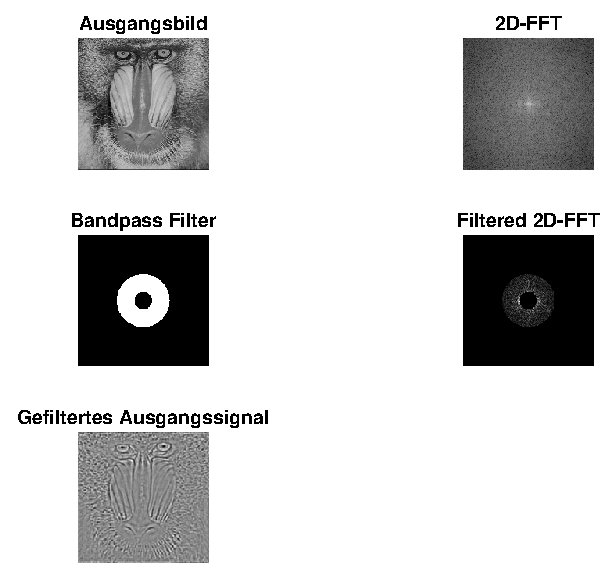
\includegraphics{fig/ex3_1.eps}
            \caption{Signals for $f_1 = 1 \si{\hertz}$}
            \label{fig:ex3_1}
        \end{figure}

        \begin{figure}
            \centering
            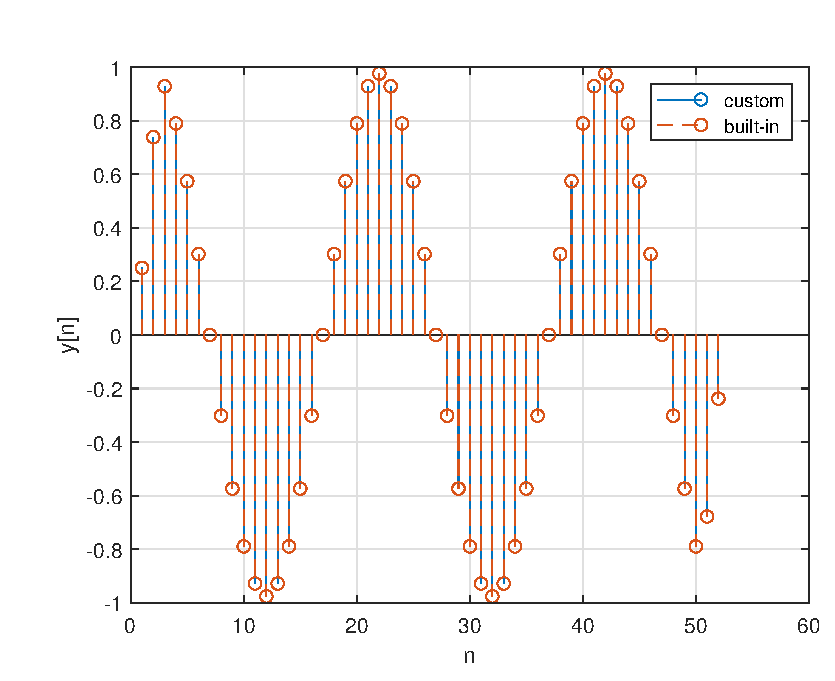
\includegraphics{fig/ex3_2.eps}
            \caption{Signals for $f_2 = 3 \si{\hertz}$}
            \label{fig:ex3_2}
        \end{figure}
    \end{enumerate}
\end{exercise}

\begin{exercise}{Linearity and Time Invariance}
    \begin{itemize}
        \item For arbitrary input signals $x_1(t)$ and $x_2(t)$ with corresponding output signals $y_1(t)$ and $y_2(t)$ let $x(t) = \alpha x_1(t) + \beta x_2(t)$ ($\alpha, \beta$ arbitrary). Then we have
        \begin{align*}
            y(t) &= (x(t))^2 = (\alpha x_1(t) + \beta x_2(t))^2 = \alpha^2x_1(t)^2 + 2 \alpha \beta x_1(t) x_2(t) + \beta^2 x_2(t)^2 \\
            &\neq \alpha y_1(t) + \beta y_2(t) = \alpha (x_1(t))^2 + \beta (x_2(t))^2
        \end{align*}
        i.e. the system is not linear. 
        
        %Sanity check: let $x_1(0) = 1$ and $x_2(0) = 2$, then $y_1(0) = 1$ and $y_2(0) = 4$. But with $x(0) = x_1(0) + x_2(0) = 3$ we have $y(0) = 9 \neq y_1(0) + y_2(0) = 5$.

        Let $x(t)$ be an arbitrary input signal with associated output signal $y(t)$. Let $x'(t)$ be a version of $x(t)$ that is shifted by arbitrary $T$, $x'(t) = x(t - T)$, with output signal $y'(t)$. Then we have
        \begin{align*}
            y'(t) = (x'(t))^2 = (x(t - T))^2 = y(t - T)
        \end{align*}
        which demonstrates time-invariance.

        \item For signals and variables as above, we have
        \begin{align*}
            y(t) &= x(t) \sin(\Omega_0 t) = (x_1(t) + y_1(t)) \sin(\Omega_0 t) = x_1(t)\sin(\Omega_0 t) + y_1(t)\sin(\Omega_0 t) \\
            &= y_1(t) + y_2(t)
        \end{align*}
        which establishes linearity. Further, we have
        \begin{align*}
            y'(t) = x'(t) \sin(\Omega_0 t) = x(t - T)\sin(\Omega_0 t) \neq y(t - T) = x(t - T) \sin(\Omega_0 (t - T))
        \end{align*}
        i.e. the system is not time-invariant.
    \end{itemize}
\end{exercise}

\end{document}
